% -*-latex-*-

\title{Orbiter Technical Notes: Earth Atmosphere Model}
\author{Martin Schweiger}
\date{March 5, 2009}

\documentclass[a4paper]{article}
\usepackage[dvips]{graphicx}
\usepackage{amsmath}
\usepackage{amsfonts}
\usepackage{amssymb}
\usepackage{times}
\usepackage{cite}

\begin{document}
\bibliographystyle{unsrt}

%\renewcommand{\vec}[1]{\ensuremath{\mathbf{#1}}}

\newcommand{\vR}[1]{\ensuremath{\vec{R}_{#1}}}
\newcommand{\nR}[1]{\ensuremath{|\vR{#1}|}}
\newcommand{\mat}[1]{\ensuremath{\mathsf{#1}}}
\newcommand{\Kelvin}{\ensuremath{\mathrm{K}}}

\maketitle

\section{Introduction}
From Edition 2009, Orbiter supports a choice of different atmosphere models for Earth. In addition to the Edition 2006 legacy model, the default distribution also contains implementations of the Jacchia model \cite{jacchia65, jacchia71, jacchia77} and the NRLMSISE-00 model which is based on the MSISE90 model.

These models address the shortcomings of the 2006 legacy model, in particular the underestimation of density and pressure above 120\,km. Both new models are valid to significantly higher altitudes (2500\,km, compared to 200\,km for the legacy model).

They provide the temperature, particle density for different molecular constituents, total mass density and molecular weight as a function of altitude, in the range from 90 to 2500\,km. For the Jacchia model, the only model parameter is the exospheric temperature, $T_\infty$, which in turn depends on various parameters, such as the relative position of the sun, geomagnetic activity, and solar flux. The NRLMSISE00 model also uses date information to compute variations on different time scales.

\section{Exospheric temperature}
Calculation of $T_\infty$ is required for applying the J77 model. The exospheric temperature is varying with time and position, and must therefore be recalculated for each new density evaluation. The model takes into account solar activity, geomagnetic activity, and a model for the diurnal variations in $T_\infty$.

The J71 model gives specifies the nighttime minimum global exosphere temperature, excluding geomagnetic activity, as
\begin{equation}
T_C = 379.0K + 3.24K \bar{F}_{10.7} + 1.3K(F_{10.7}-\bar{F}_{10.7})
\end{equation}
where $F_{10.7}$ is the daily average solar flux value one day prior, measured at wavelength 10.7\,cm, and $\bar{F}_{10.7}$ is the average value over three solar rotations of 27 days. Units for solar flux values are given in Solar Flux Units of $10^{-22}\,W/(m^2 Hz)$.

In Orbiter, solar flux values based on observations are not taken into account. Instead, a constant flux of
\begin{equation}
F_{10.7} = \bar{F}_{10.7} = 140 \cdot 10^{-22} W/(m^2 Hz)
\end{equation}
is assumed, which reduces the expression for $T_C$ to
\begin{equation}
T_C = 832.6K
\end{equation}
The diurnal model for $T_\infty$ takes into account the local hour angle of the sun with respect to the measurement point, as well as the declination of the sun and the geographic latitude of the measurement point. This model is given by
\begin{equation}
T_1 = T_C \left[ 1 + 0.3 \left( \sin^{2.2}|\theta| + (\cos^{2.2}|\eta| - \sin^{2.2}|\theta|) \cos^{3.0}(\tau/2) \right) \right]
\end{equation}
with
\begin{eqnarray}
\tau &=& H - 37.0^\circ + 6.0^\circ \sin(H+43.0^\circ) \\
\theta &=& \frac{1}{2} (\varphi + \delta_\odot ) \\
\eta &=& \frac{1}{2} (\varphi - \delta_\odot)
\end{eqnarray}
where $\delta_\odot$ denotes the sun's declination, $\varphi$ is the geographic latitude and $H$ the hour angle of the sun with respect to the measurement point, given by
\begin{equation}
H = \alpha - \alpha_\odot
\end{equation}
where $\alpha$ and $\alpha_\odot$ are the right ascension of the measurement point and the sun, respectively.

Finally, geomagnetic activity is taken into account by the Jacchia model by specifying a modification term $\Delta T_\infty$ for $T_\infty$ in the form
\begin{eqnarray}
\Delta T^H_\infty &=& 28.0\Kelvin \cdot K_p + 0.03\Kelvin e^{K_p}\qquad (z > 350\,km) \\
\Delta T^L_\infty &=& 14.0\Kelvin \cdot K_p + 0.02\Kelvin e^{K_p}\qquad (z < 350\,km)
\end{eqnarray}
for two separate altitude regimes, respectively. $K_p$ is the three-hourly planetary geomagnetic index for a time 6.7 hours previous. To provide continuity at z=350\,km, a transition function $f$ is introduced:
\begin{equation}
f = \frac{1}{2} (\tanh(0.04 (z - 350\,km)) + 1)
\end{equation}
The geomagnetic activity correction $\Delta T_\infty$ can then be written as
\begin{equation}
\Delta T_\infty = f \Delta T^H_\infty + (1-f) \Delta T^L_\infty
\end{equation}
In Orbiter, variations in geomagnetic activity are ignored. Instead, a constant geomagnetic index of $K_p = 3.0$ is assumed. This simplifies the correction terms to
\begin{eqnarray}
\Delta T^H_\infty &=& 84.6026\Kelvin \\
\Delta T^L_\infty &=& 42.4017\Kelvin \\
\Delta T_\infty &=& (42.2009 f + 42.4017)\Kelvin
\end{eqnarray}
The final value for the exospheric temperature is then given by
\begin{equation}
T_\infty = T_1 + \Delta T_\infty
\end{equation}
Examples for global distributions of $T_\infty$ are shown in Fig.~\ref{fig:t_infty}, for two different solar declination values ($0^\circ$ and $20^\circ$). Note that the maximum of $T_\infty$ is trailing the Sun's location (indicated by a circle).

\begin{figure}
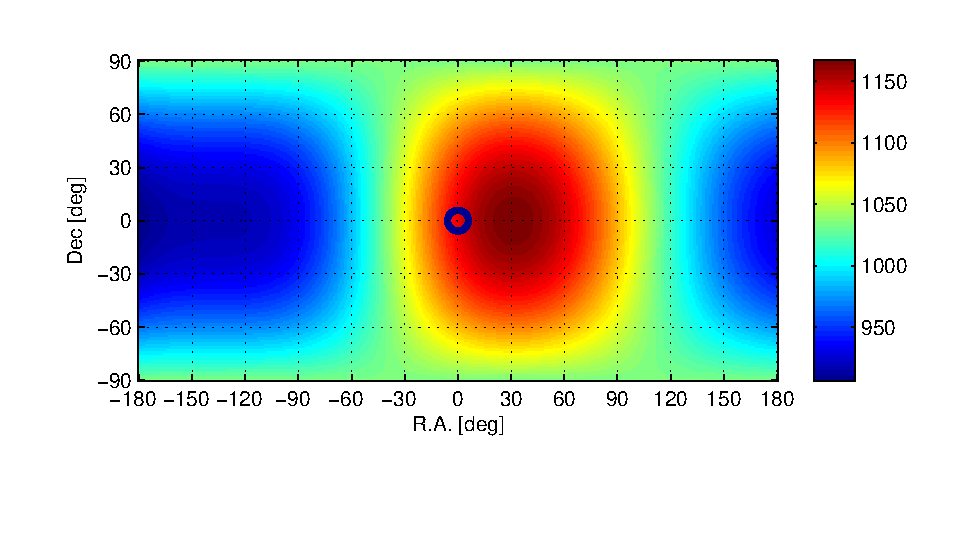
\includegraphics[width=0.8\textwidth]{exotemp1.eps}
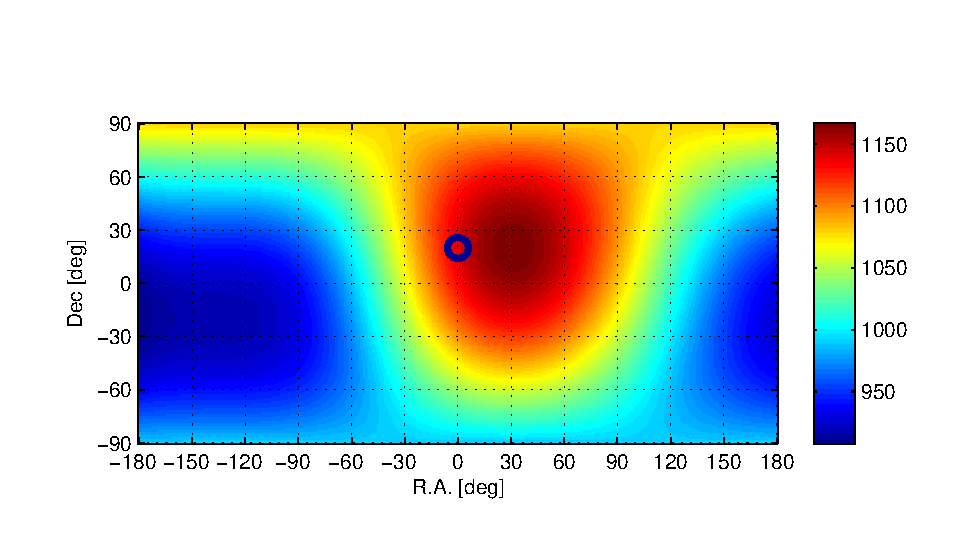
\includegraphics[width=0.8\textwidth]{exotemp2.eps}
\caption{Exospheric temperature distributions as a function of geographic longitude and latitude, for two different declination values of the Sun: $0^\circ$ (top) and $20^\circ$ (bottom). The position of the sun is indicated by a circle.}
\label{fig:t_infty}
\end{figure}

\section{The Jacchia temperature and density model}
The Jacchia model is static and assumes two distinct altitude regimes, where in the lower regime (from 90 to 100\,km) the atmospheric constituents are mixed, and the density is computed by integrating the barometric equation. At altitudes $> 100$\,km, the atmosphere is assumed to be in diffusion equilibrium for each of the individual constituents.

\subsection{Temperature}
The temperature profile obtained from the Jacchia code as a function of altitude for three different values of $T_\infty$ is shown in Fig.~\ref{fig:jacchia_temp}. As can be seen, the temperature profiles are identical up to an altitude of about 100\,km, where the standard US atmospheric model is used. At higher altitudes, the temperatures asymdotically approach the prescribed exospheric temperature.

\begin{figure}
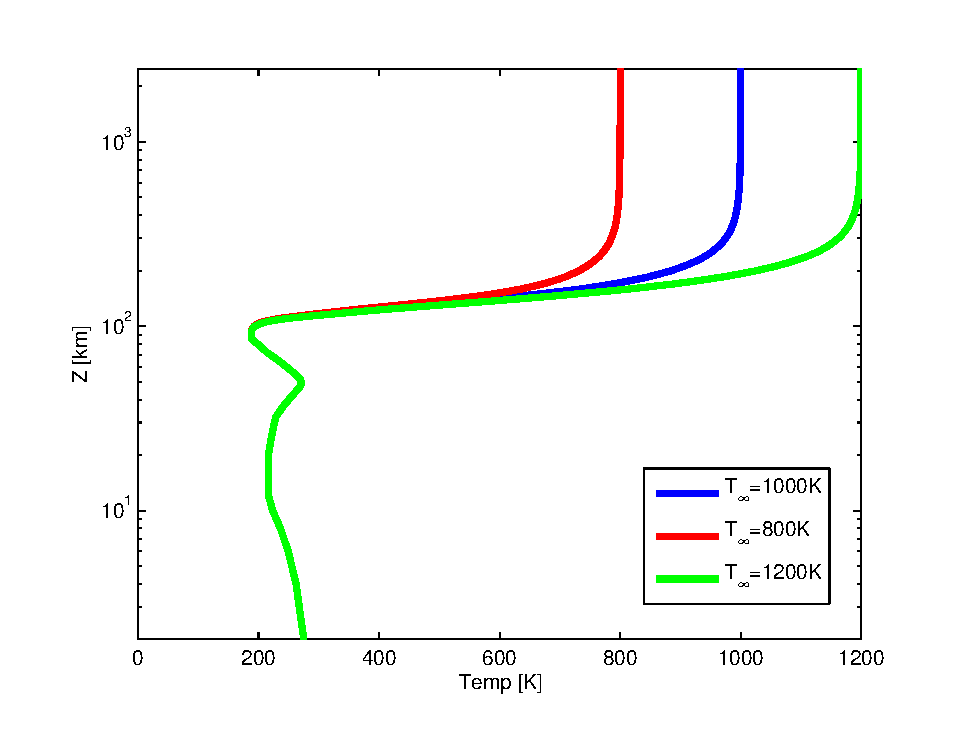
\includegraphics[width=0.8\textwidth]{jacchia_temp.eps}
\caption{J77 temperature profiles as a function of altitude for different values of exospheric temperature $T_\infty$.}
\label{fig:jacchia_temp}
\end{figure}

\subsection{Density}

The Jacchia model requires the integration of a barometric or diffusion equation up to the desired altitude. This method is not computationally efficient if density values at arbitrary altitudes are required. In this case, a reasonable compromise between computational speed and accuracy can be achieved by precomputing lookup tables over the required ranges of altitude $z$ and exospheric temperature $T_\infty$, and interpolating to the actual parameters. Alternatively, a basis expansion in the two parameters can be used. Gill~\cite{gill96} has approximated the J71 density model (denoted here by J71G) by a bi-polynomial expansion of the form
\begin{equation}\label{eq:interpol}
\log \rho(z,T_\infty) = \sum_{i=0}^m \sum_{j=0}^n c_{ij} z^i T_\infty^j
\end{equation}
where $c_{ij}$ are the basis coefficients of the expansion obtained by a least-squares optimisation.

To provide sufficient accuracy while keeping the expansion to a reasonably low order, the temperature and altitude range was divided into sub-regions, and separate basis expansions calculated for each of them. Continuity of the density values and derivatives across region boundaries was ensured by applying appropriate constraints to the least squares fits. The authors present the coefficients for a basis expansion using a 5th degree polynomial in temperature and 6th degree polynomial in altitude for each region.

The density profiles as a function of altitude for three values of $T_\infty$ are shown in Fig.~\ref{fig:dens} for both the J77 and the J71G models.
\begin{figure}
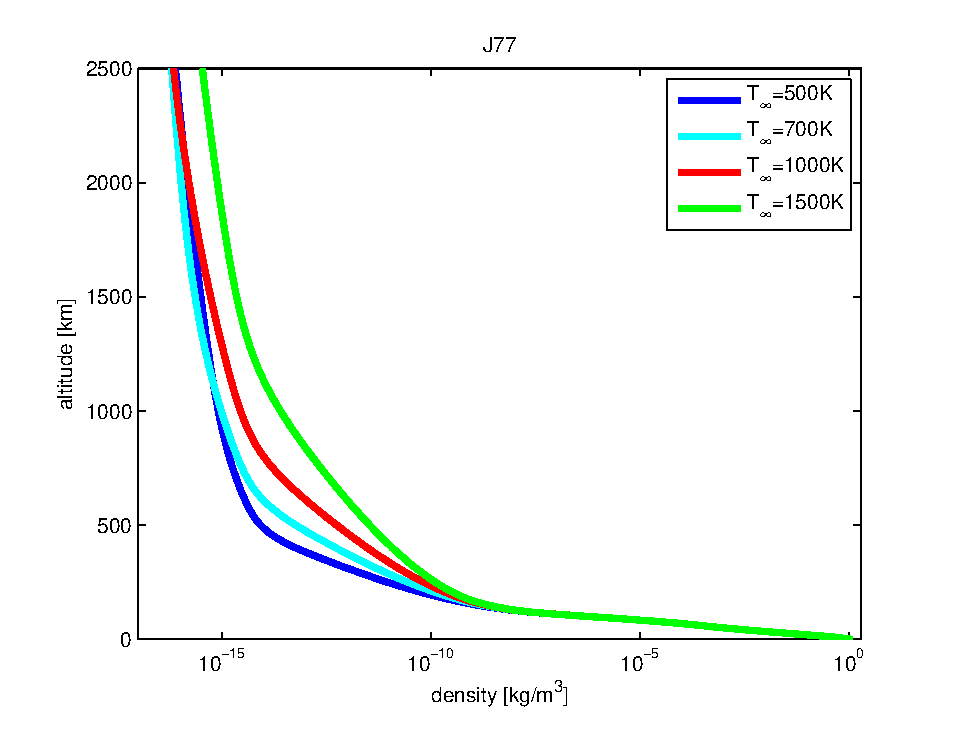
\includegraphics[width=0.5\textwidth]{dens_j77.eps}
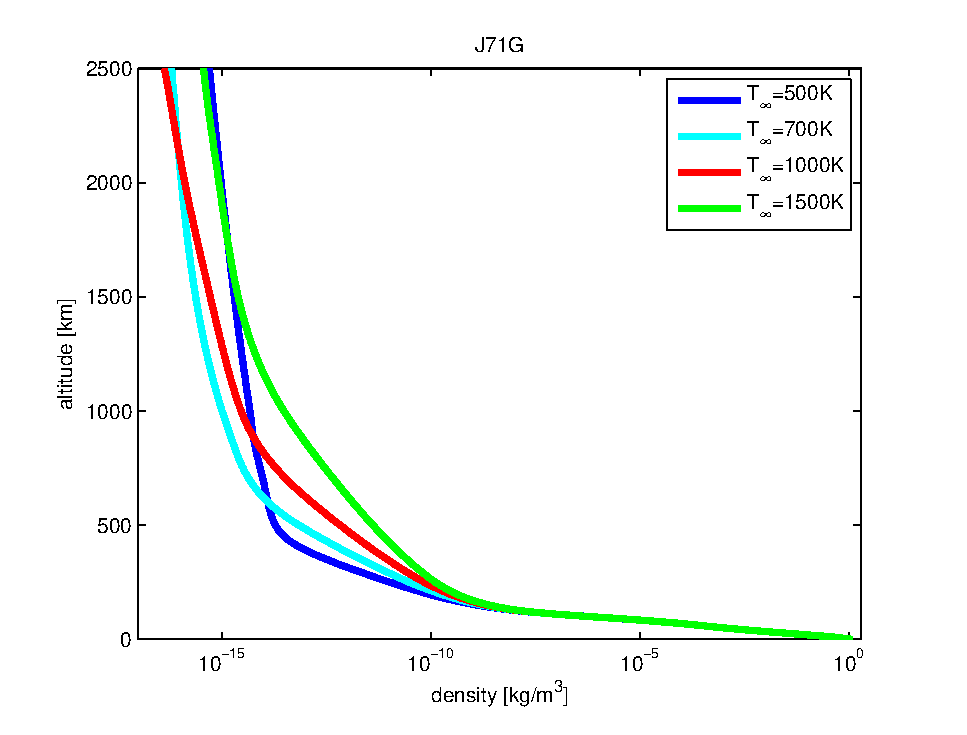
\includegraphics[width=0.5\textwidth]{dens_j71g.eps}
\caption{Density profiles for the J77 (left) and J71G model (right) as a function of altitude, for three different values of the exospheric temperature.}
\label{fig:dens}
\end{figure}
The relative difference between the two models is shown in Fig.~\ref{fig:denserr}. It can be seen that the models agree well for medium to high values of $T_\infty$, but diverge significantly for low values. This may be caused by the fact that the interpolated Gill solution is modelling the earlier J71 model rather than J77, so may reflect the difference between the underlying models, rather than an effect of the interpolation approach. As can be seen in the right image, the models only diverge below temperatures of 600\,K, which are not encountered in Orbiter's model for $T_\infty$.
\begin{figure}
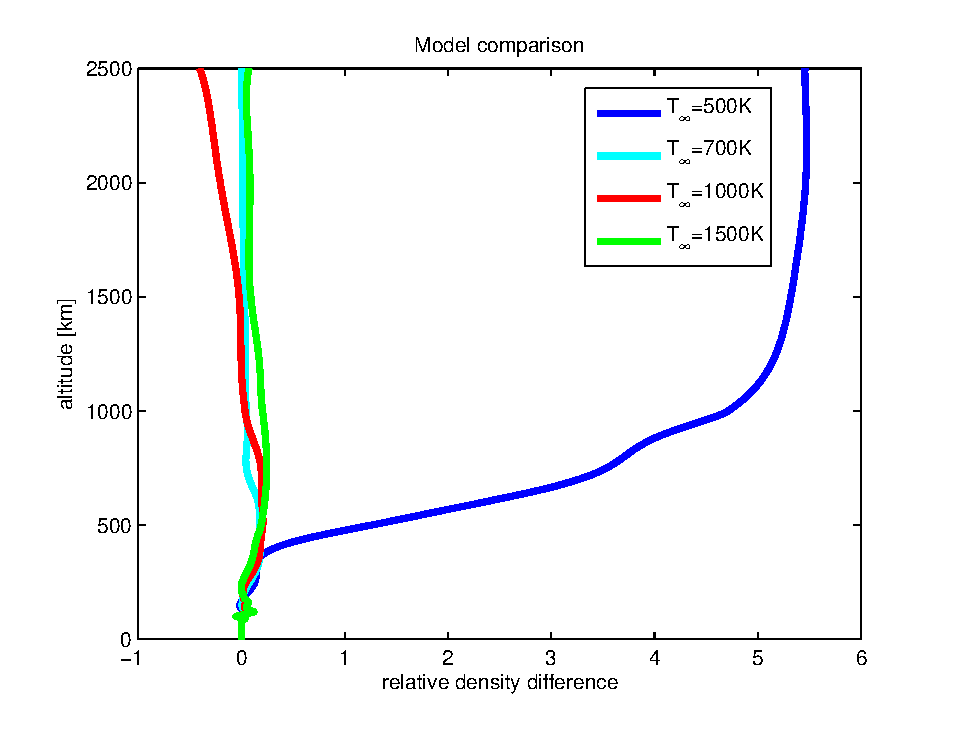
\includegraphics[width=0.5\textwidth]{dens_relerr.eps}
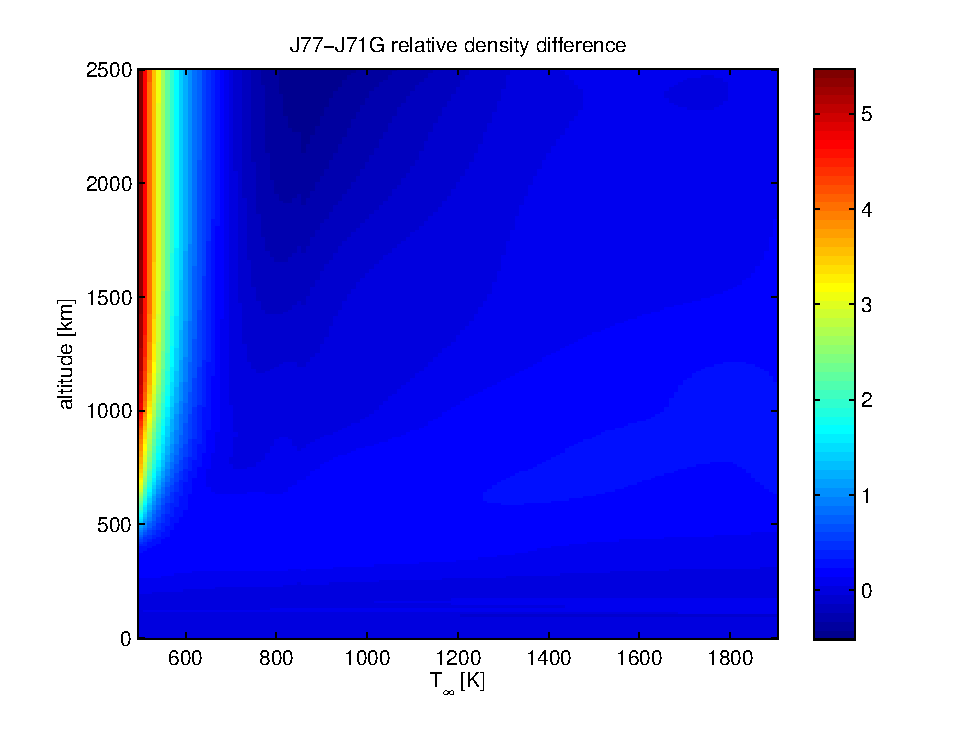
\includegraphics[width=0.5\textwidth]{dens_relerr2.eps}
\caption{Relative difference between the J77 and J71G models as a function of altitude, for three different values of the exospheric temperature (left), and for the full temperature range (right).}
\label{fig:denserr}
\end{figure}

\subsection{Pressure}
 
We obtain atmospheric pressure from density by applying the ideal gas law
\begin{equation}
p = \rho_N k T
\end{equation}
where $\rho_N$ [m$^{-3}$] is the particle density, and $k$ [J/K] is the Boltzmann constant. However, while the original Jacchia model returns $\rho_N$, the interpolated Jacchia-Gill model instead provides the mass density $\rho$. The relationship between $\rho$ and $\rho_N$ is given by
\begin{equation}
\rho_N = \rho \frac{N_A}{M}
\end{equation}
where $N_A$ is Avogadro's constant and $M$ is the molar mass of the gas mixture. The Jacchia model does provide $M$, but as with the density, this requires an expensive numerical integration over altitude. Therefore I present here a polynomial series approximation of $M$ in the parameters $z$ and $T_\infty$ similar to the density expansion of the Jacchia-Gill model (Eq.~\ref{eq:interpol}). Instead of a piecewise patched solution, the parameter range of $90\,km \leq z \leq 2500\,km$ and $500\,K \leq T_\infty \leq 1900\,K$ is mapped with a single series of order 8 in $z$ and order 4 in $T_\infty$. The basis coefficients $c^{(M)}$ were obtained by a least-squares fit and $c$ are listed in Appendix A. The distribution of the interpolation solution of $M$ is shown in Fig.~\ref{fig:molmass}. Below $z=90$\,km the value of $M$ is derived from the US standard atmosphere model.

\begin{figure}
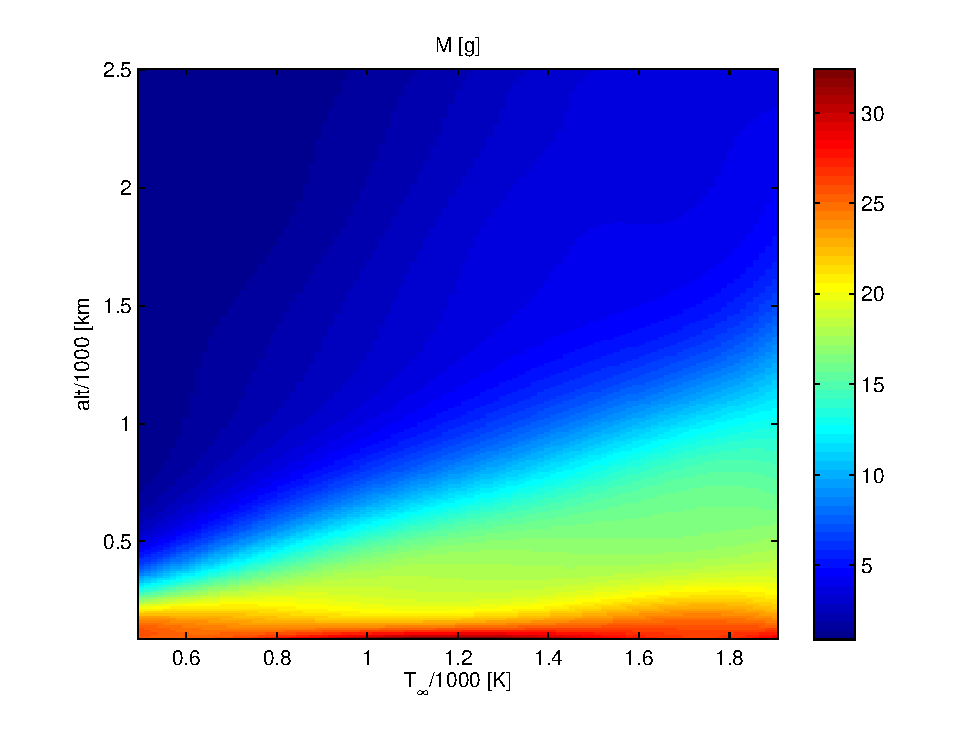
\includegraphics[width=0.5\textwidth]{molmass.eps}
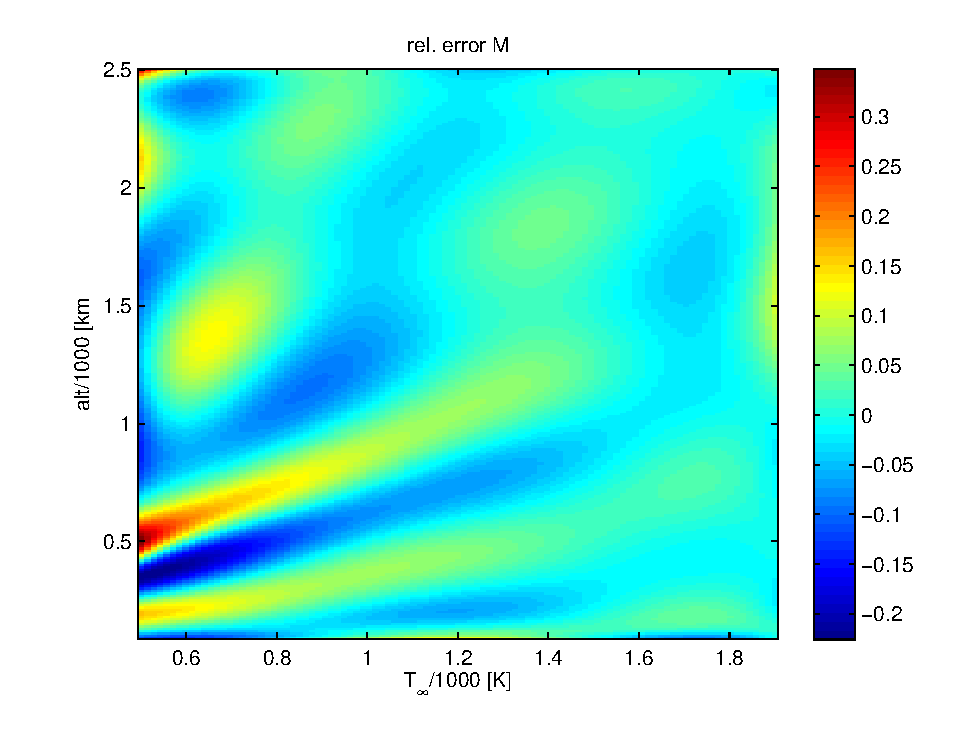
\includegraphics[width=0.5\textwidth]{molmass_err.eps}
\caption{Left: Distribution of molar mass as a function of altitude and exospheric temperature, obtained from a polynomial series expansion. Right: relative error of the series solution compared to the original Jacchia model data.}
\label{fig:molmass}
\end{figure}
The atmospheric pressure values calculated with the J77 model and with the J71G model augmented with the molecular weight interpolation as outlined above are shown in Fig.~\ref{fig:pressure}. The differences between the two models at low values of $T_\infty$ observed for density naturally also appear for the pressure values. Above 600\,K the agreement is very good.

\begin{figure}
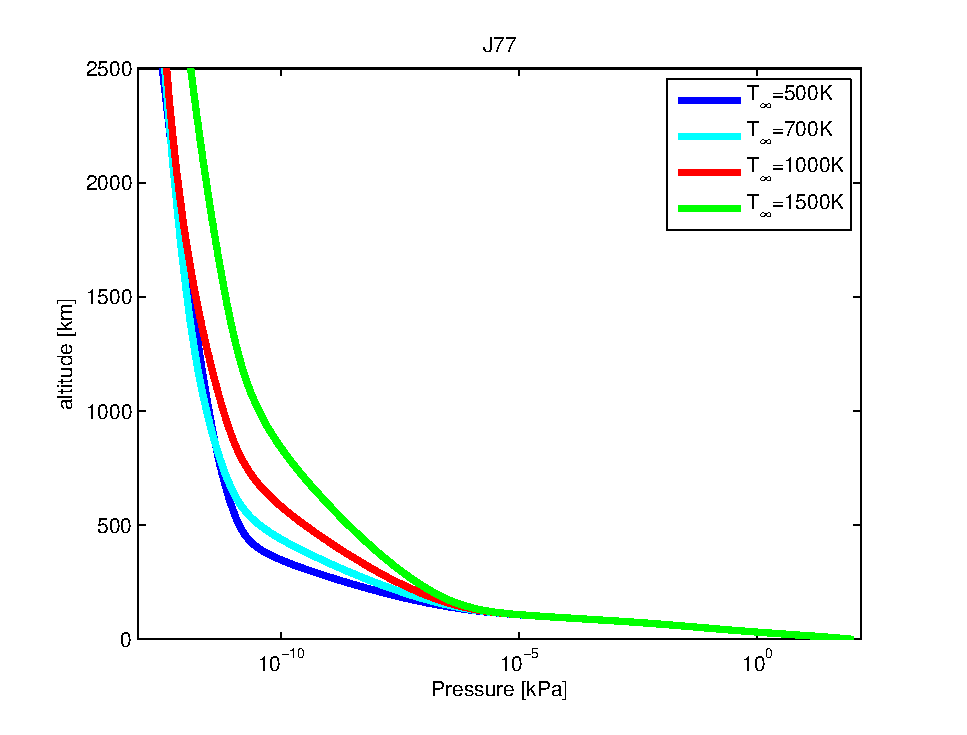
\includegraphics[width=0.5\textwidth]{prs_j77.eps}
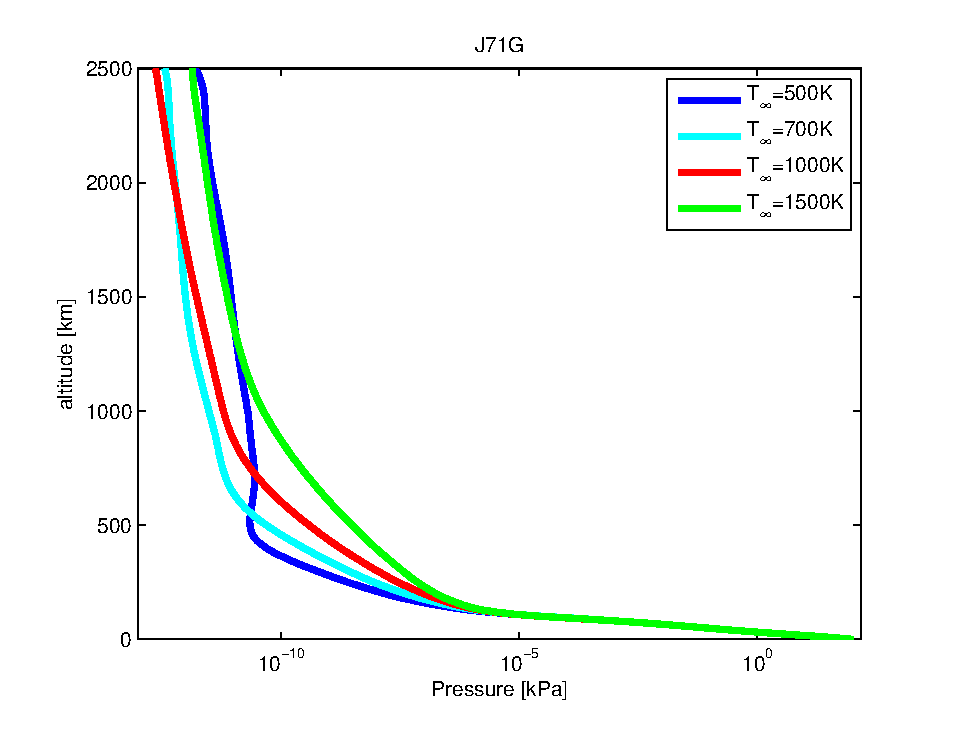
\includegraphics[width=0.5\textwidth]{prs_j71g.eps}
\caption{Pressure profiles for the J77 (left) and the augmented J71G model (right) as a function of altitude, for three different values of the exospheric temperature.}
\label{fig:pressure}
\end{figure}

\section{The NRLMSISE-00 atmosphere model}
A further atmospheric model supported by Orbiter is the NRLMSISE-00 model, developed by Picone, Hedin and Drob, with a C version by D. Brodowski. It is based on the MSISE90 model, adding some further observation data. MSISE90 provides the neutral temperature and density from ground level to thermospheric altitudes. Unlike the Jacchia models, the low-altitude data are not static, but vary with location. They are based on the MAP Handbook (Labitzke et al. 1985) tabulation of zonal average temperature and pressure by Barnett and Corney. Below 20 km these data were supplemented with averages from the National Meteorological Center (NMC). In addition, pitot tube, falling sphere, and grenade sounder rocket measurements from 1947 to 1972 were taken into consideration. Above 72.5 km MSISE-90 is essentially a revised MSIS-86 model taking into account data derived from space shuttle flights and newer incoherent scatter results.

The input parameters for the NRLMSISE-00 model are altitude, geodetic longitude and latitude, day of year, seconds in day, average and current F10.7 flux, and magnetic index. On output, the model provides temperature at altitude, exospheric temperature, total mass density, and number densities for He, O, N$_2$, O$_2$, Ar, H, N and anomalous oxygen.

The algorithm for calculating $T_\infty$ differs between the J71G and the NRLMSISE-00 model. Figure~\ref{fig:comp_tinfty} compares the $T_\infty$ profiles over a single day (left) and over a year, at UT=0 and UT=12 hours (right). It can be seen that the daily profile of the NRLMSISE-00 model appears more complex, showing less symmetry and a pronounced minimum. The annual NRLMSISE-00 profile displays a higher amplitude and lower average than the J71G model.

\begin{figure}
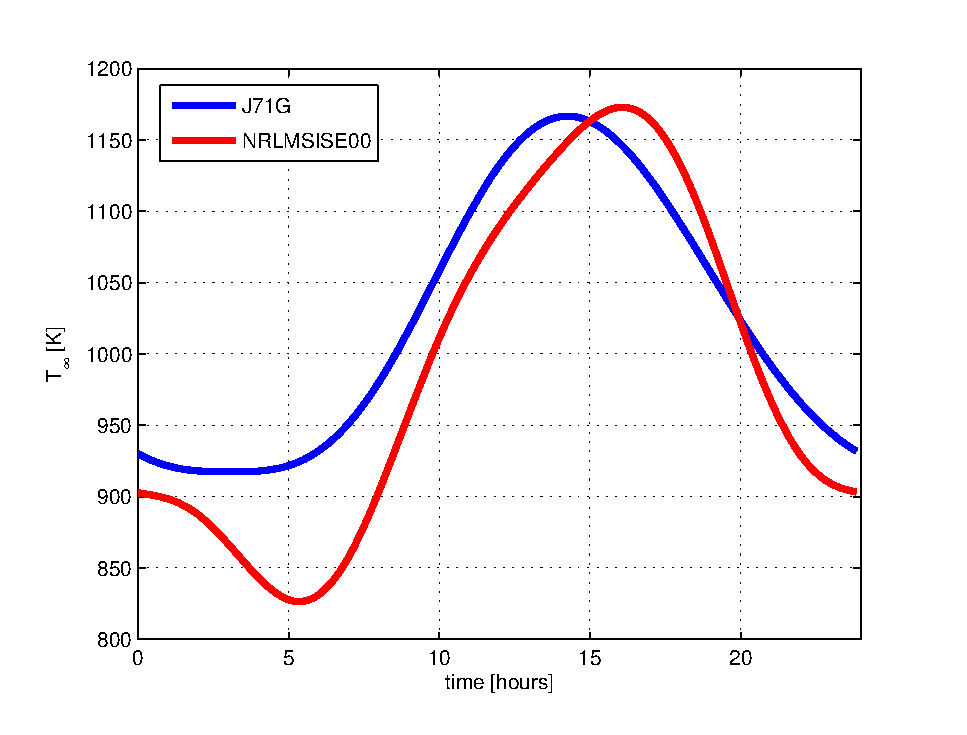
\includegraphics[width=0.5\textwidth]{tinf_daily.eps}
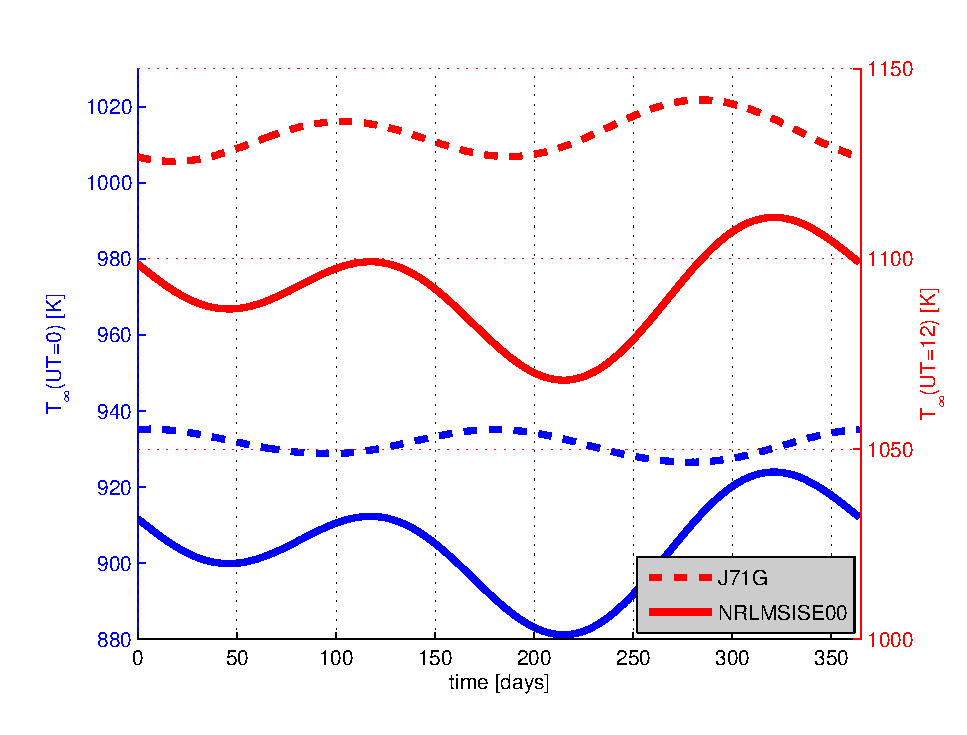
\includegraphics[width=0.5\textwidth]{tinf_annual.eps}
\caption{Comparison of $T_\infty$ values for the J71G and NRLMSISE-00 models. Left: daily profile on 10 March. Right: annual profile, measured daily at UT=0 and UT=12 hours. For all data, a location of longitude=0 and latitude=0 was used.}
\label{fig:comp_tinfty}
\end{figure}

The temperature profile as a function of altitude for a given data (MJD 54900.5) at latitude=0, longitude=0) for both models is shown in Fig.~\ref{fig:comp_t}.
\begin{figure}
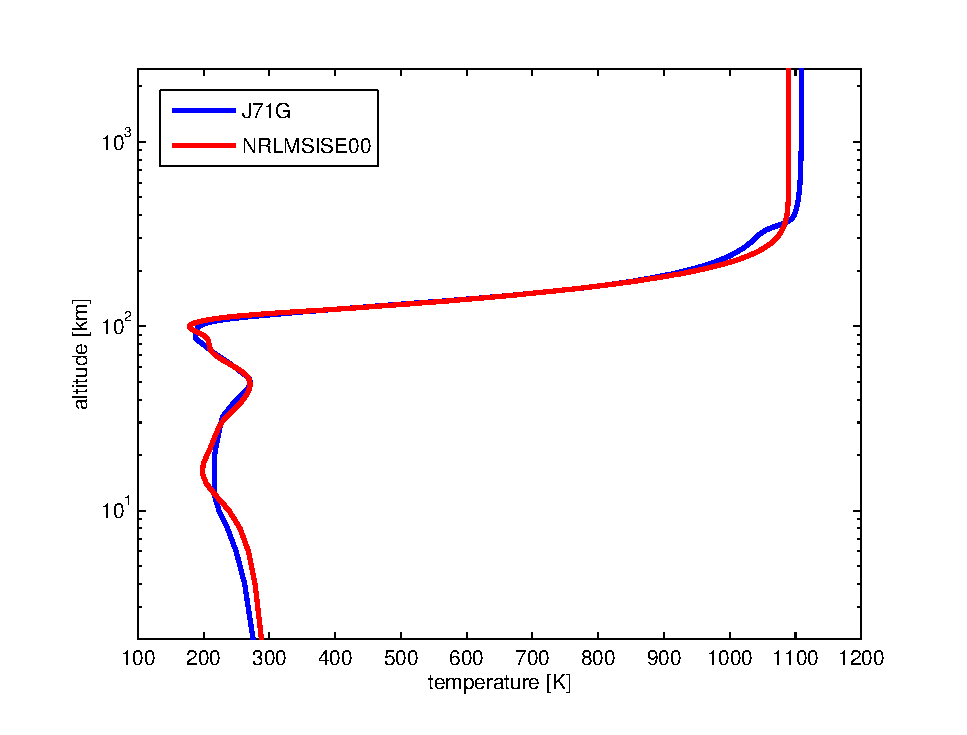
\includegraphics[width=0.5\textwidth]{j71g_nrlmsise00_cmp1.eps}
\caption{Comparison of temperature altitude profiles of J71G and NRLMSISE-00 at MJD=54900.5, longitude=0, latitude=0.}
\label{fig:comp_t}
\end{figure}
The density and pressure altitude profiles for both models at the same time and location are shown in Fig.~\ref{fig:comp_dns_p}. It can be seen that the models generally agree well.
\begin{figure}
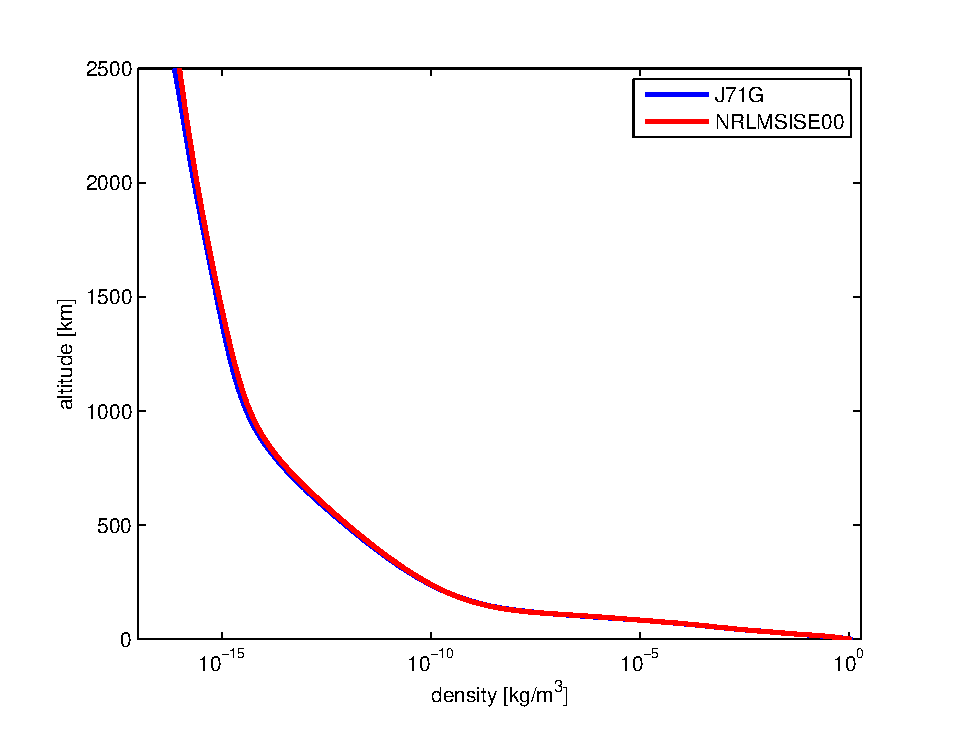
\includegraphics[width=0.5\textwidth]{j71g_nrlmsise00_cmp2.eps}
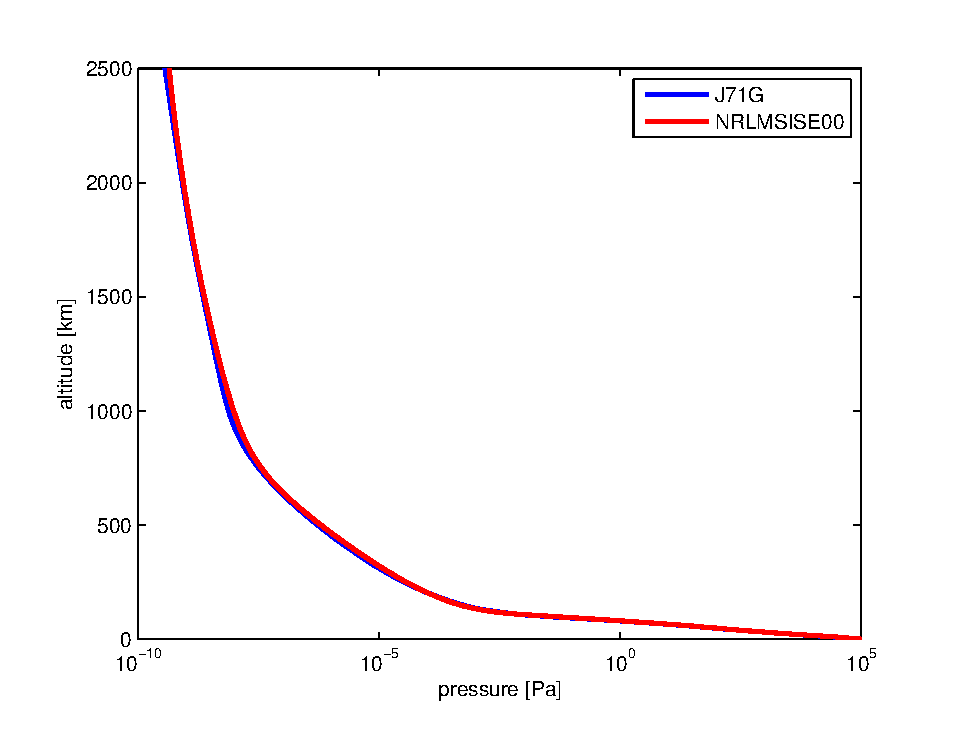
\includegraphics[width=0.5\textwidth]{j71g_nrlmsise00_cmp3.eps}
\caption{Comparison of density and pressure altitude profiles of J71G and NRLMSISE-00 at MJD=54900.5, longitude=0, latitude=0.}
\label{fig:comp_dns_p}
\end{figure}

\section{Comparison with Orbiter 2006 legacy model}
The atmosphere model in Orbiter Edition 2006 (denoted as OB06) uses a simple static, piecewise linear temperature profile. For segments of constant temperature, pressure and density are calculated as
\begin{equation}
p(z)=p_1 e^{-[g_0/(RT)](z-z_1)}, \qquad \rho(z)=\rho_1 e^{-[g_0/(RT)](z-z_1)},
\end{equation}
where $z_1$ is the base altitude of the segment, $p_1$ and $\rho_1$ are the corresponding pressure and density, $R$ is the specific gas constant, set to $R=286.91$\,JK$^{-1}$kg$^{-1}$ for air, and $g_0$ is the gravitational acceleration.
The pressure and density in sections of linearly varying temperature are calculated as
\begin{equation}
p(z)=p_1\left[\frac{T(z)}{T_1}\right]^{-g_0/(aR)},\qquad
\rho(z)=\rho_1\left[\frac{T(z)}{T_1}\right]^{-[(g_0/(aR))+1]}
\end{equation}
where $a$ is the temperature gradient [K/m].

Because the gravitational acceleration $g$ cannot be assumed constant over the altitude range, altitude $z$ must be interpreted as a \emph{geopotential} altitude. Conversion between geometric altiude $z_G$ and geopotential altitude $z$ is given by
\begin{equation}
h = \frac{R}{R+z_g}z_g
\end{equation}
where $R$ is the planet radius.

Similar to the J71G model, OB06 is based on a static standard atmosphere model at low altitudes (below 105\,km). Above this altitude, up to 200\,km, the temperature is assumed to be constant at 225.66\,K. This is equivalent to a very low value of $T_\infty$, and consequently the temperature profiles of the two models diverge rapidly between the two models above 120\,km for more realistic values of $T_\infty$, as shown in Fig.~\ref{fig:ob_j71g_temp}, where a value of $T_\infty=1000$\,K was chosen for the J71G model.

\begin{figure}
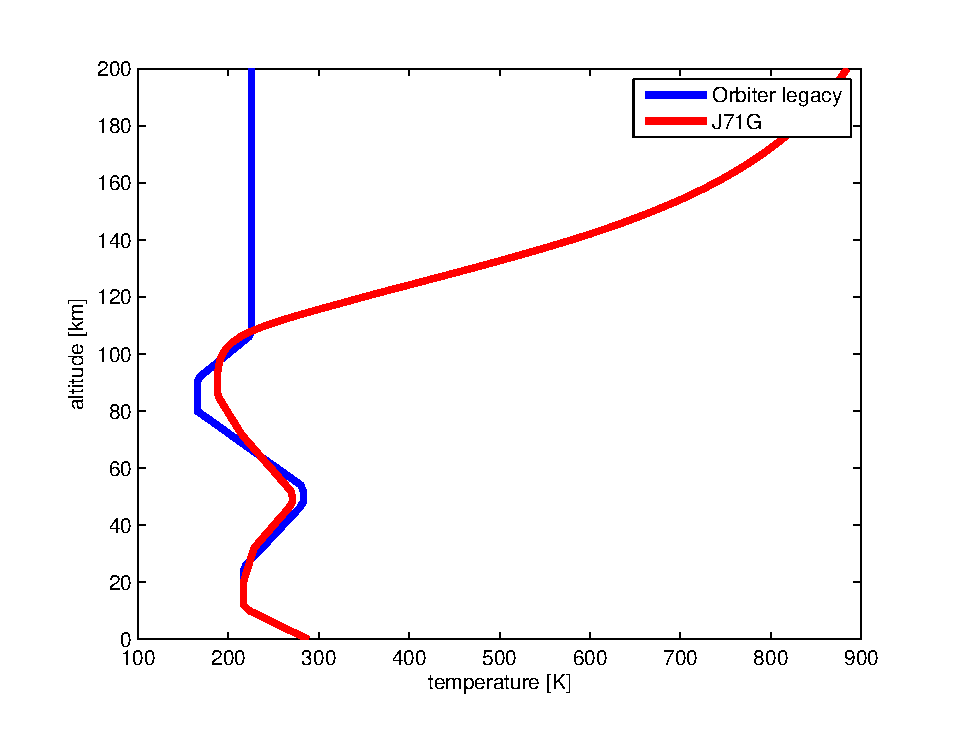
\includegraphics[width=0.5\textwidth]{ob_j71g_temp.eps}
\caption{Comparison of temperature distributions between the Orbiter legacy model and the J71G model for $T_\infty=1000$\,K.}
\label{fig:ob_j71g_temp}
\end{figure}
Likewise, the pressure and density profiles of the legacy Orbiter model agree well with the J71G model below 120\,km, while at higher altitudes the Orbiter model continues to follow an exponential decay, while the J71G model maintains significantly higher density and pressure values (Fig.~\ref{fig:ob_j71g_dens_prs}).
As a result, the OB06 model values drop to essentially insignificant values at $z=200$\,km, the default cutoff altitude of the legacy model, while density and pressure remain significant to much higher altitudes for the J71G model.

The transition from the OB06 to the J71G model in Orbiter will therefore lead to significantly higher drag effects from altitudes above 120\,km which will continue substantially above the previous cutoff altitude of 200\,km.

\begin{figure}
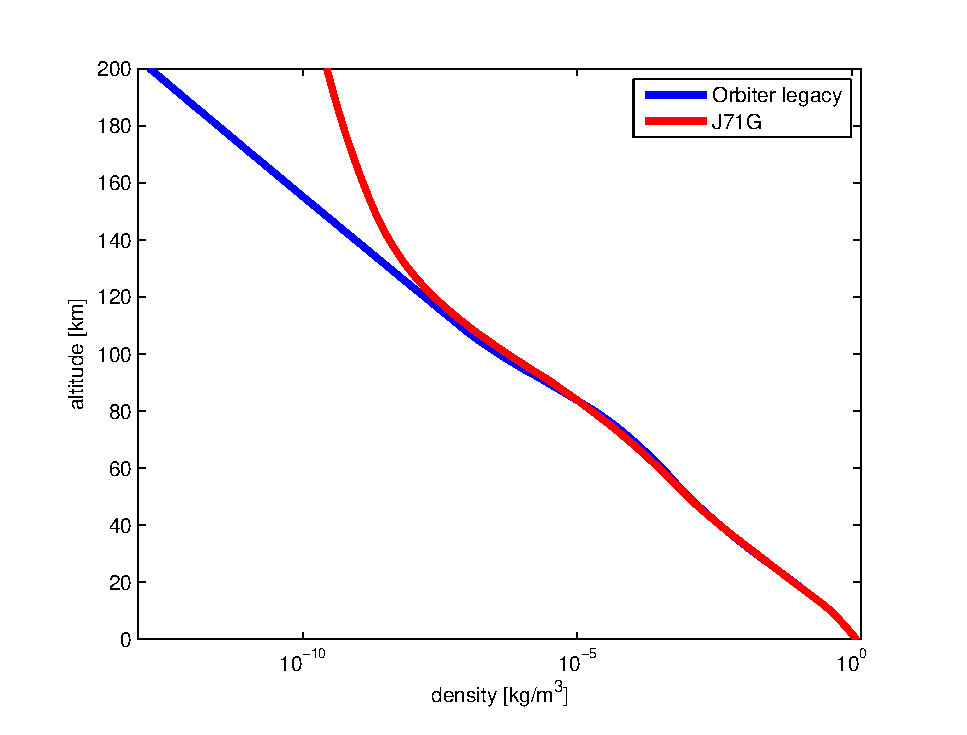
\includegraphics[width=0.5\textwidth]{ob_j71g_dens.eps}
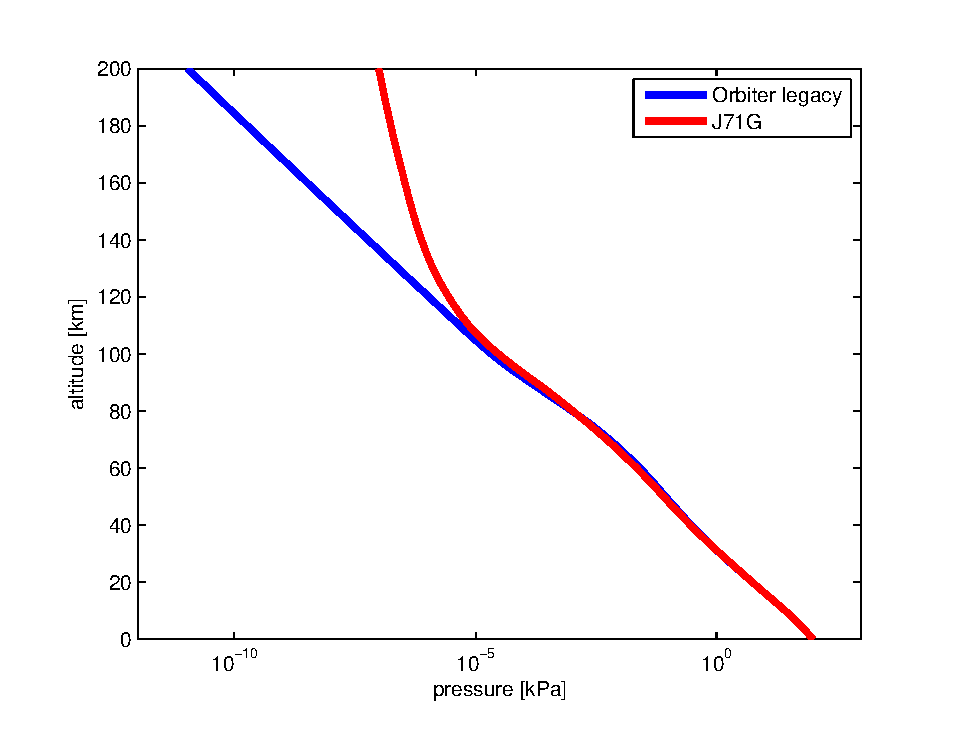
\includegraphics[width=0.5\textwidth]{ob_j71g_prs.eps}
\caption{Comparison of density (left) and pressure distributions (right) between the Orbiter legacy model and the J71G model for $T_\infty=1000$\,K.}
\label{fig:ob_j71g_dens_prs}
\end{figure}

\section {Computational complexity}
For a real-time application like Orbiter, the computational efficiency of the atmosphere model is important. Atmosphere data are queried at each time frame by each vessel within the atmosphere range limit of a given celestial body. For densely populated simulation scenarios, a complex atmosphere model may adversely affect performance.

Timing results for the three atmosphere models are shown in Table~\ref{tab:timing}. They show the times for 1000 evaluations of model evaluation at different altitudes. It can be seen that the NRLMSISE-00 model is significantly more expensive than the J71G model by approximately an order of magnitude, and both models are substantially more expensive than the trivial Orbiter legacy model.

It should however be noted that for moderately loaded simulation scenarios, even the more expensive models may not significantly degrade performance. For a test scenario with 50 vessels in the atmosphere, the application of the NRLMSISE-00 model resulted in a drop in frame rate from 130 to 114 frames per second.
\begin{table}
\begin{tabular}{l|lll}
Altitude [km] & 50 & 150 & 1000 \\ \hline
2006 Legacy model & 0.000055 & 0.000056 & - \\
J71G model & 0.000289 & 0.0015 & 0.0020 \\
NRLMSISE-00 model & 0.00384 & 0.0266 & 0.0146
\end{tabular}
\caption{Timing comparison between atmosphere models: Times for 1000 model evaluations at different altitudes.}
\label{tab:timing}
\end{table}

\bibliography{../ref}

\section*{Appendix A}
Basis coefficients $c^{(M)}_{ij}$ for obtaining the logarithmic molar mass $M$ of the atmospheric gas mixture as a function of altitude $z$ (in units of km/1000) and exospheric temperature $T_\infty$ (in units of K/1000).
\begin{equation}
\log_{10}(M(z,T_\infty)) \approx \sum_{i=0}^8 \sum_{j=0}^4 c^{(M)}_{ij} z^i T_\infty^j
\end{equation}
\footnotesize
\begin{tabular}{r|rrrrr}
i/j & 0 & 1 & 2 & 3 & 4 \\ \hline
0 &  3.60906627e+00 & -1.35761290e+01 &  2.55465982e+01 & -1.77204699e+01 &  4.07696683e+00 \\
1 & -1.35606636e+01 &  1.29084956e+02 & -2.84612534e+02 &  2.12822504e+02 & -5.11308350e+01 \\
2 & -1.25207810e+01 & -3.19579690e+02 &  9.77718751e+02 & -8.21851276e+02 &  2.09837747e+02 \\
3 &  6.98268484e+01 &  4.02801988e+02 & -1.69988881e+03 &  1.57164796e+03 & -4.21561534e+02 \\
4 & -8.44186988e+01 & -2.88755547e+02 &  1.67090876e+03 & -1.67274401e+03 &  4.67667119e+02 \\
5 &  4.42735679e+01 &  1.24592950e+02 & -9.68963604e+02 &  1.03850337e+03 & -3.01006087e+02 \\
6 & -7.92712088e+00 & -3.81200493e+01 &  3.34875778e+02 & -3.77385160e+02 &  1.12634338e+02 \\
7 & -1.14988223e+00 &  9.20028301e+00 & -6.52157331e+01 &  7.51024325e+01 & -2.28683127e+01 \\
8 &  4.13670214e-01 & -1.18725773e+00 &  5.60433585e+00 & -6.36983671e+00 &  1.95706136e+00
\end{tabular}

\end{document}
